\documentclass[final]{beamer}

\usepackage[size=custom, width=100, height = 200, scale=1.4,debug]{beamerposter}

\usetheme{Pittsburgh}

\definecolor{orange}{RGB}{243,112,33}
\definecolor{blue}{RGB}{0,84,150}
\setbeamercolor{block title}{fg=orange,bg=white} % Colors of the block titles
\setbeamercolor{block body}{fg=black,bg=white} % Colors of the body of blocks
\setbeamercolor{block alerted title}{fg=white,bg=dblue!70} % Colors of the highlighted block titles
\setbeamercolor{block alerted body}{fg=black,bg=dblue!10} % Colors of the body of highlighted blocks
% Many more colors are available for use in beamerthemeconfposter.sty

%-----------------------------------------------------------
% Define the column widths and overall poster size
% To set effective sepwid, onecolwid and twocolwid values, first choose how many columns you want and how much separation you want between columns
% In this template, the separation width chosen is 0.024 of the paper width and a 4-column layout
% onecolwid should therefore be (1-(# of columns+1)*sepwid)/# of columns e.g. (1-(4+1)*0.024)/4 = 0.22
% Set twocolwid to be (2*onecolwid)+sepwid = 0.464
% Set threecolwid to be (3*onecolwid)+2*sepwid = 0.708

\newlength{\sepwid}
\newlength{\onecolwid}
\newlength{\twocolwid}
\newlength{\threecolwid}
\setlength{\paperwidth}{100cm} %  EPS page sizes
\setlength{\paperheight}{200cm} %
\setlength{\sepwid}{0.024\paperwidth} % Separation width (white space) between columns
\setlength{\onecolwid}{0.31\paperwidth} % Width of one column
\setlength{\twocolwid}{0.62\paperwidth} % Width of two columns
\setlength{\topmargin}{-1.5in} % Reduce the top margin size
%-----------------------------------------------------------

\usepackage{qrcode}
\usepackage{graphicx}  % Required for including images
\graphicspath{./fig}

\usepackage{booktabs} % Top and bottom rules for tables


\begin{document}

\addtobeamertemplate{block end}{}{\vspace*{2ex}} % White space under blocks
\addtobeamertemplate{block alerted end}{}{\vspace*{2ex}} % White space under highlighted (alert) blocks

\setlength{\belowcaptionskip}{2ex} % White space under figures
\setlength\belowdisplayshortskip{2ex} % White space under equations

\begin{frame}[t] % The whole poster is enclosed in one beamer frame

%----------------------------------------------------------------------------------------
%	TITLE SECTION
%----------------------------------------------------------------------------------------

\begin{center}
    \begin{Huge}
        \rule{\linewidth}{0.25cm}
        \textsc{%textsc makes text small capsx1%aQ$&kSPmV
        \color{orange}{Magnetic Nulls from the Topological Perspective}}\\
    \end{Huge}

    \begin{large}
        \textsc{Christopher Berg Smiet$^{1,2,\dagger}$, Ben Israeli$^{1}$, Amitava Bhattacharjee$^{1,2}$}\\
        \color{orange}{$^1$Princeton Plasma Physics Laboratory, Princeton, 08540 NJ, USA}, \color{blue}{$^\dagger$ csmiet@pppl.gov}\\
    \color{orange}{$^2$Leiden University, Leiden, 2300 RA, Netherlands}\\

    \end{large}
\end{center}
\rule{\linewidth}{0.3cm}




%----------------------------------------------------------------------------------------


\begin{columns}[t] % The whole poster consists of two major columns, the second of which is split into two columns twice - the [t] option aligns each column's content to the top

\begin{column}{\sepwid}\end{column} % Empty spacer column

\begin{column}{\twocolwid} % The first column
\begin{columns}[t,totalwidth=\twocolwid] % Split up the two columns wide column

\begin{column}{\onecolwid}\vspace{-.6in} % The first column within column 1 (column 1.1)

%----------------------------------------------------------------------------------------
%	THE INDEX OF A NULL
%----------------------------------------------------------------------------------------
\begin{block}{Introduction}
	Three-dimensional magnetic nulls play an important role in astrophysical
	plasma physics and earth-based fusion concepts such as the FRC. 
	We present a novel method of conceptualizing the movement of these nulls in
	three-dimensional fields. 
	We define the concept of isotropes (iso=same, tropos = direction), lines in space
	along which the magnetic field points in the same direction. 
	It is shown that the isotropes can be recovered as the stream lines of
	the isotropic field, which is defined via a geometric formula from the
	magnetic field.
	
\end{block}


\begin{block}{The topological Index of a 3D null}
    Let $\mathbf{B}(\mathbf{x}): \mathbb{R}^3\rightarrow \mathbb{R}^3$ be a continuous
    vector field.
    Define the map $g:\mathbb{R}^3\rightarrow S^2$ that sends points in
    space to the unit vectors in the direction of the field $\mathbf{B}$
    (i.e. points on the unit sphere).
    \begin{equation}\label{eq:director}
        g = \frac{\mathbf{B}(\mathbf{x})}{|\mathbf{B}(\mathbf{x})|}
    \end{equation}
    The topological index of an isolated null $x_0$ of $\mathbf{B}$ is given by
    the degree of the mapping $g|_{\partial D^3_{x_0}}$ restricted to the surface of
    a solid sphere containing only the null, to the unit sphere:
    \begin{equation}\label{eq:index1}
        \mathrm{Ind}(x_0)=\mathrm{Deg}(g|_{partial D^3_{x_0}})
    \end{equation}
    The degree of a mapping counts how many times the domain wraps around the range.
    The degree of any map between spheres is always in
    $\mathbb{Z}$~\cite{brouwer1911abbildung}, therefore:
    $\mathrm{Deg}(g|_{\partial D^3})\in\mathbb{Z}$.
    If $D^3$ contains more than one isolated zero, then the following theorem holds:
    \begin{equation}\label{eq:indextheorem}
        \mathrm{Deg}(g|_{\partial D^3})= \sum_{x_0\in D^3} \mathrm{Ind}(x_0)
    \end{equation}
    The degree is a homotopy invariant, and can be used to locate nulls in a volume by
    bisection~\cite{greene1992locating}.

\end{block}It is shown that the isotropes can 
be recovered as the stream lines of the isotropic field, which is defined 
via a geometric formula from the magnetic field.

%----------------------------------------------------------------------------------------

\end{column} % End of column 2.1

\begin{column}{\onecolwid}\vspace{-.6in} % The second column within column 2 (column 2.2)

%----------------------------------------------------------------------------------------
%	METHODS
%----------------------------------------------------------------------------------------

\begin{block}{Type-A and Type-B nulls}
    Magnetic nulls are usually classified into Type-A (negative) or Type-B (positive)~\cite{lau1990three, parnell1996structure, greene1988geometrical}.
    These names are derived from considering the matrix of partial derivatives of the
    field at the null:
    \begin{equation}\label{eq:matrix}
        \mathsf{M}_{ij}= \partial_j B_i.
    \end{equation}
    Since $\nabla\cdot\mathbf{B}=0$, $\mathrm{Tr}(\mathsf{M})=0$.
    Type-A nulls have two positive and one negative element on the diagonal, Type-B nulls
    two negative, one positive.
    The calculation of the topological index of Type-A and Type-B nulls with the matrices:
    \begin{equation}
        \mathsf{M}_A = \begin{bmatrix} 0.5 & 0&0 \\ 0 & 0.5 & 0 \\
        0&0& -1  \end{bmatrix}.
        \quad
        \mathsf{M}_B = \begin{bmatrix} -0.5 & 0&0 \\ 0 & -.5 & 0 \\
        0&0& 1  \end{bmatrix}.
    \end{equation}
\begin{columns}[t,totalwidth=\onecolwid] % Split up the two columns wide column
    \begin{column}{.45\onecolwid}
        \begin{centering}
        \textbf{Type-A}
        \begin{figure}
        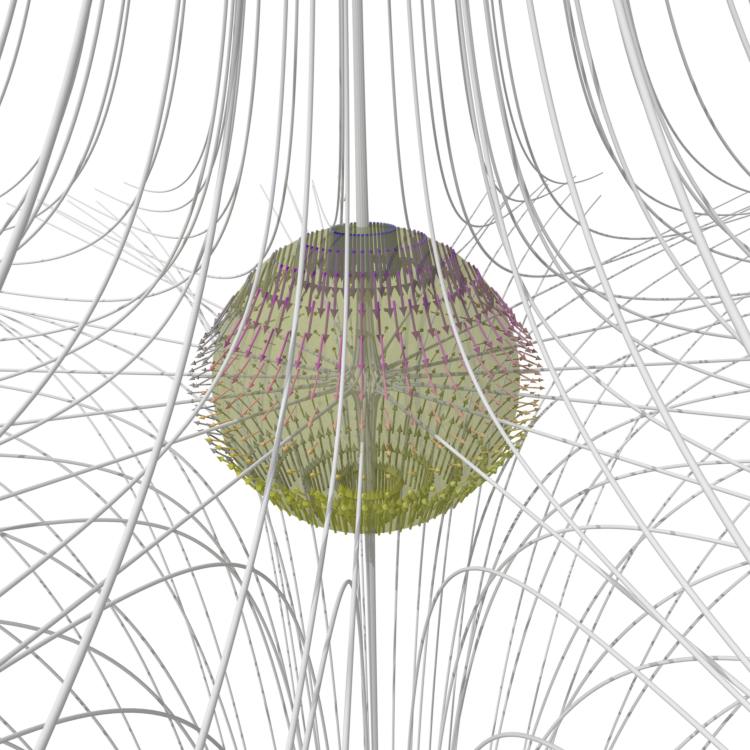
\includegraphics[width=.45\onecolwid]{fig/negindex_start.png}
        \end{figure}
        $\downarrow$
        \begin{figure}
        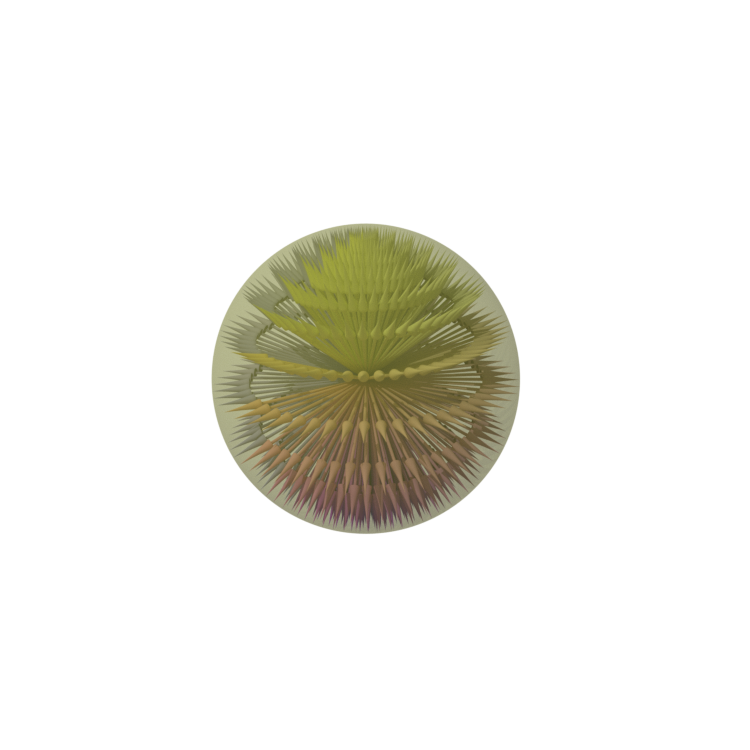
\includegraphics[width=.45\onecolwid]{fig/negindex_end.png}
        \end{figure}
        \hfil$\mathrm{Ind}(x_0)=-1 \leqno$\hfil
        \end{centering}
    \end{column}

    \begin{column}{.45\onecolwid}
        \begin{centering}
        \textbf{Type-B}
        \begin{figure}
        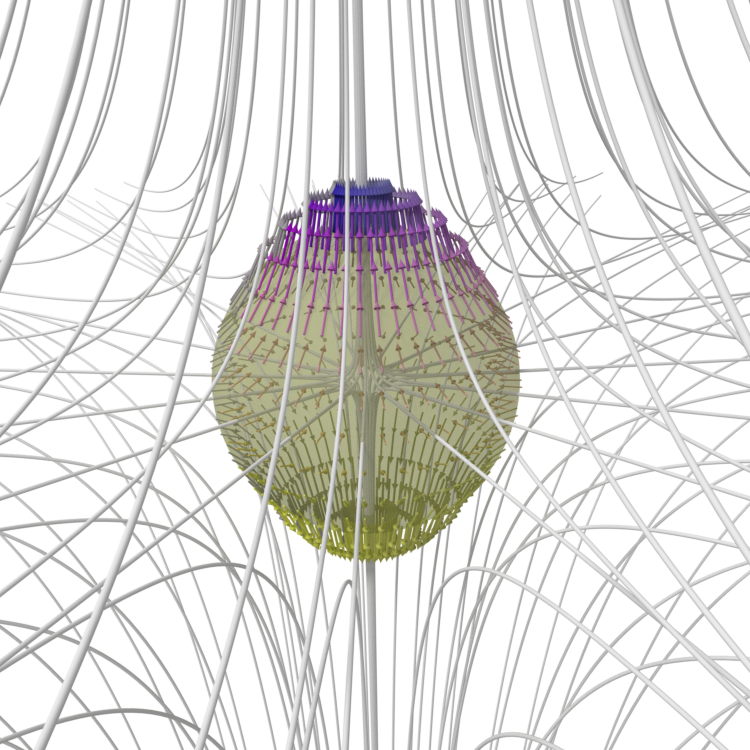
\includegraphics[width=.45\onecolwid]{fig/posindex_start.png}
        \end{figure}
        $\downarrow$
        \begin{figure}
        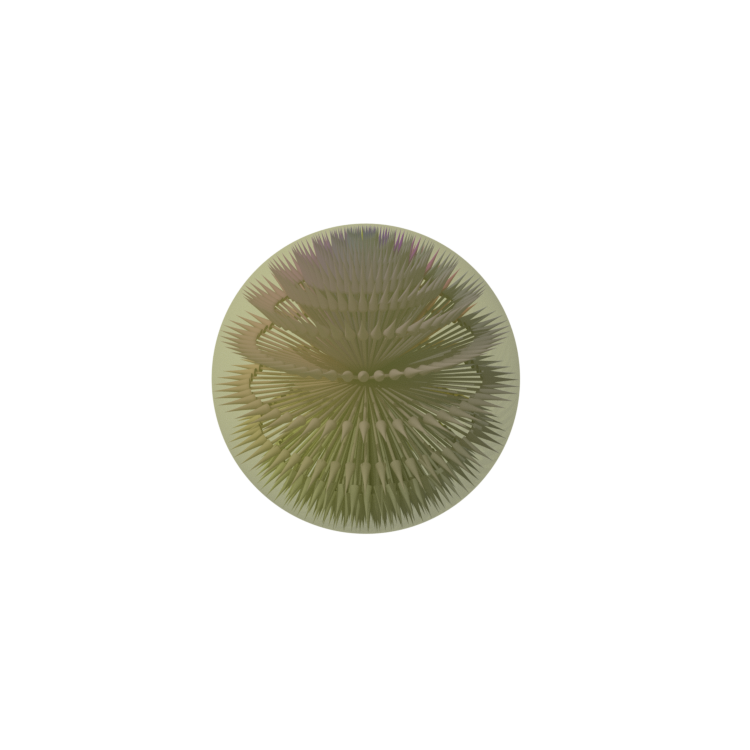
\includegraphics[width=.45\onecolwid]{fig/posindex_end.png}
        \end{figure}
        \hfil$\mathrm{Ind}(x_0)=+1 \leqno$\hfil
    \end{centering}
    \end{column}
\end{columns}

\end{block}

%----------------------------------------------------------------------------------------

\end{column} % End of column 2.2

\end{columns} % End of the split of column 2 - any content after this will now take up 2 columns width
%----------------------------------------------------------------------------------------
%	THE NULLS AROUND A DIPOLE
%----------------------------------------------------------------------------------------

\begin{block}{The Isotropes of a dipole}
    A dipole field has topological index 0, and its isotropes are straight lines passing through
	the singularity of the dipole. 
	The image below shows the magnetic field lines of a dipole given by
	\begin{equation}
		\mathbf{B} = \frac{2(\mathbf{m}\cdot\hat{\mathbf{r}})\hat{\mathbf{r}}-\mathbf{m}}
		{r^3}
	\end{equation}
	where $\mathbf{m}$ is the dipole moment given by a unit vector in the
	$\hat{z}$-direction. 
	The magnetic field lines are given by the blue curves
	Seven isotropes are shown in different colors, with a vector indicating the diretion of the
	isotrope. 
    \begin{figure}
        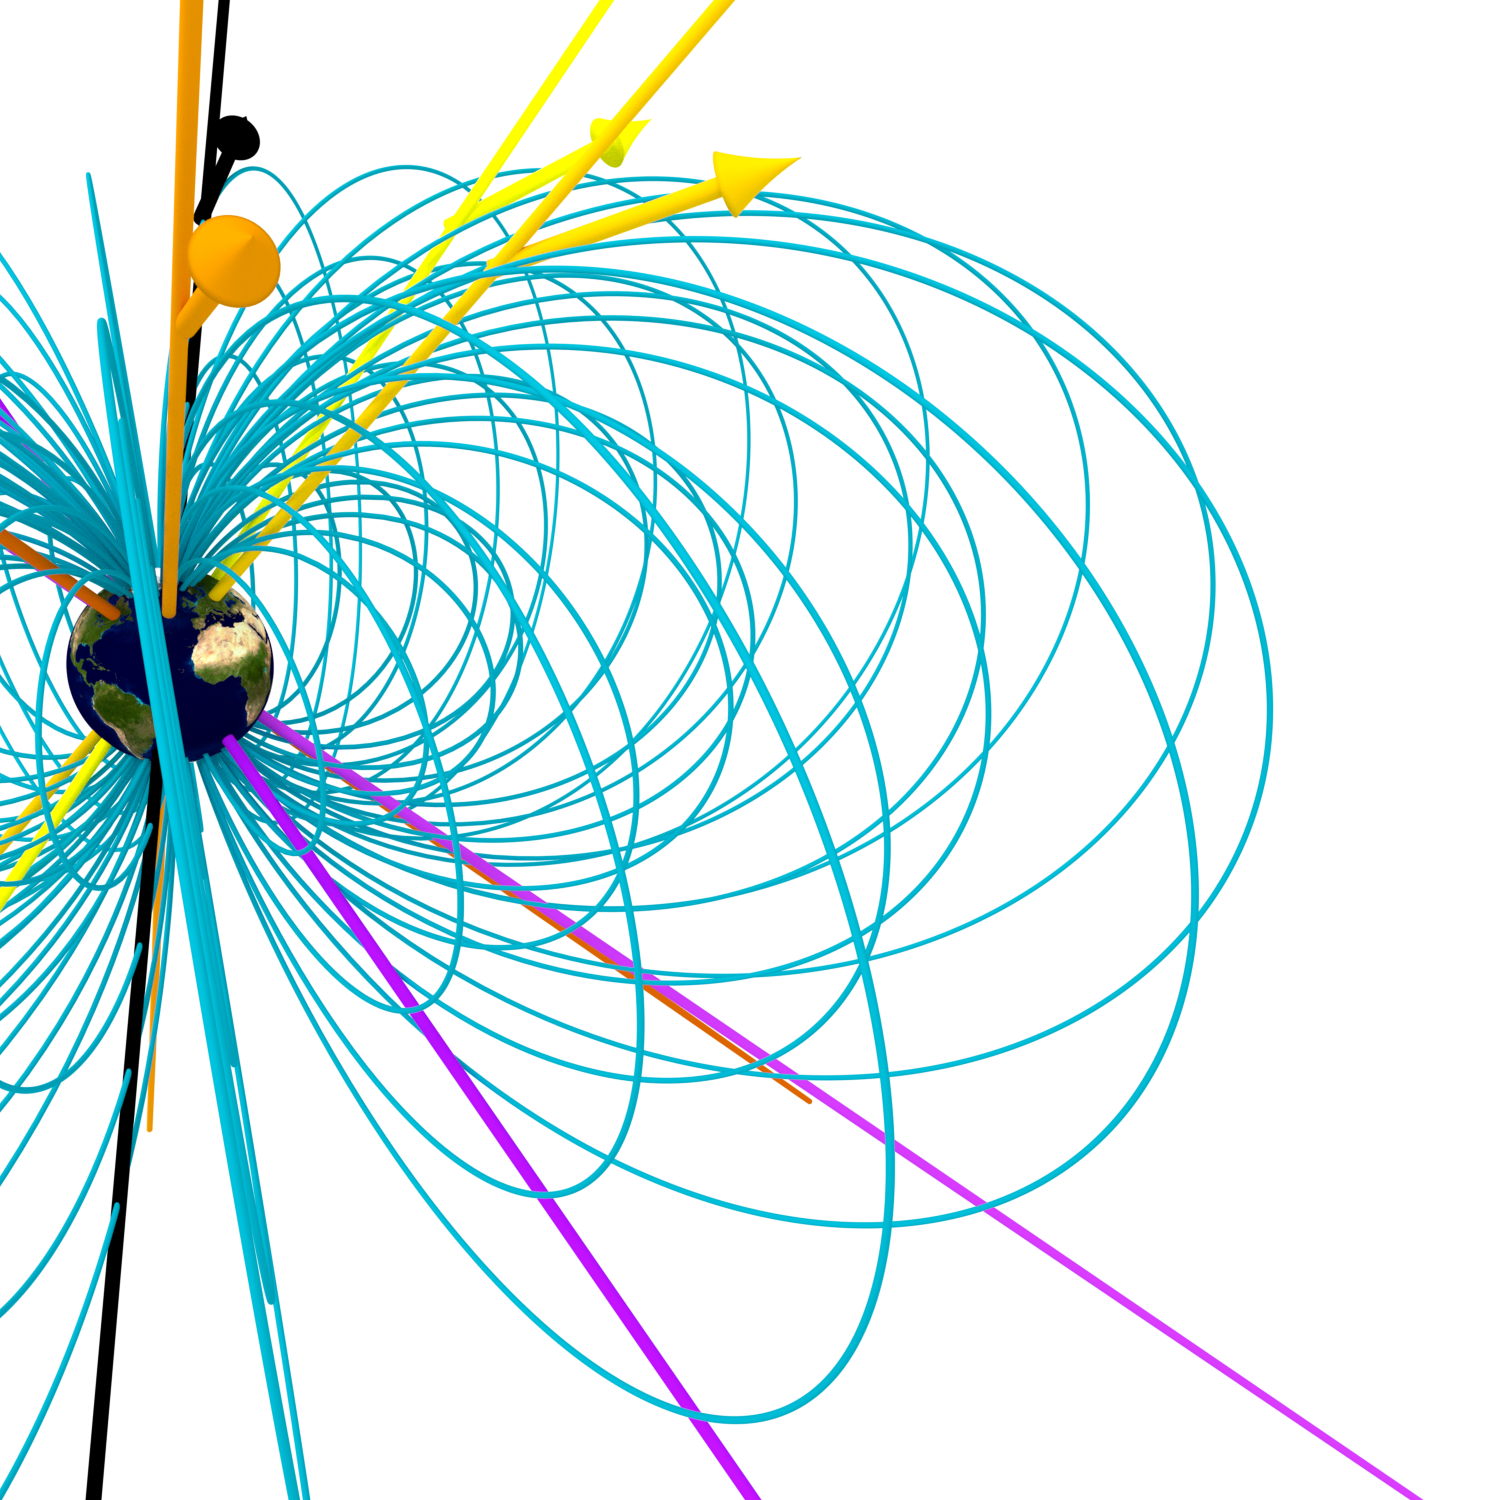
\includegraphics[width=\twocolwid]{fig/mainfig.png}
    \end{figure}
	The surfaces of constant field strength enclose the dipole. 
	Whenever a dipole is embedded in a guide field, two nulls appear where the isotrope of
	opposite direction to the guide field intersects the surface of constant magnitude
	equal to the guide field strength. 
\end{block}

%----------------------------------------------------------------------------------------
\begin{columns}[t,totalwidth=\twocolwid] % Split up the two columns wide column again

\begin{column}{\onecolwid} % The first column within column 2 (column 2.1)

%----------------------------------------------------------------------------------------
%	MATHEMATICAL SECTION
%----------------------------------------------------------------------------------------
\begin{block}{Movement of nulls}
    A topological null of index $\pm 1$ cannot be removed unless it meets with a null of opposite index. 
    The change of the magnetic field at the location of the null can be evaluated through:
    \begin{equation}
        \frac{\partial \mathbf{B}}{\partial t} = \eta \nabla^2 \mathbf{B}.
    \end{equation}
    This vector equation gives the rate and direction of change of the field at the null.
    After a finite time the field has changed, and this can be seen as adding a guide
    field in this direction to the field of the null at time 0. 
    The null will move along the isotrope corresponding to this direction.

\end{block}


\begin{block}{Topological attraction and repulsion}
    Nulls with index $n$ higher than 1 or lower than -1 are very unstable.  The degree of
    the mapping $g|_\partial D^3_{x_0}$ is $n$, therefore $S^2$, the space of
    directions is multiply covered for any ball enclosing $x_0$. 
    This means that for any direction $|n|$ isotropes approach the null arbitrarily
    closely. 

    Any change in the field at the location of the null can be seen as 
    adding a guide field to it. 
    This change will split up the null into $|n|$ copies of the nulls moving along the
    isotropes of the direction of the change. 

    When two nulls of opposite index are close, the isotropes leaving the null of positive
    index enter the null of negative index. 
    If there are only two nulls, and the field at sufficient distance is a constant field,
    then every isotrope except the one corresponding to opposite the field at infinity
    will leave one null and enter the other. 
    Any guide field (except the one mentioned above) will move the nulls along the
    corresponding isotrope until they meet. 
\end{block}

%----------------------------------------------------------------------------------------

\end{column} % End of column 2.1

\begin{column}{\onecolwid} % The second column within column 1 (column 1.2)

%----------------------------------------------------------------------------------------
%	Dipole in a guide field
%----------------------------------------------------------------------------------------
\begin{block}{The Dipole in a guide field}
    \begin{figure}
    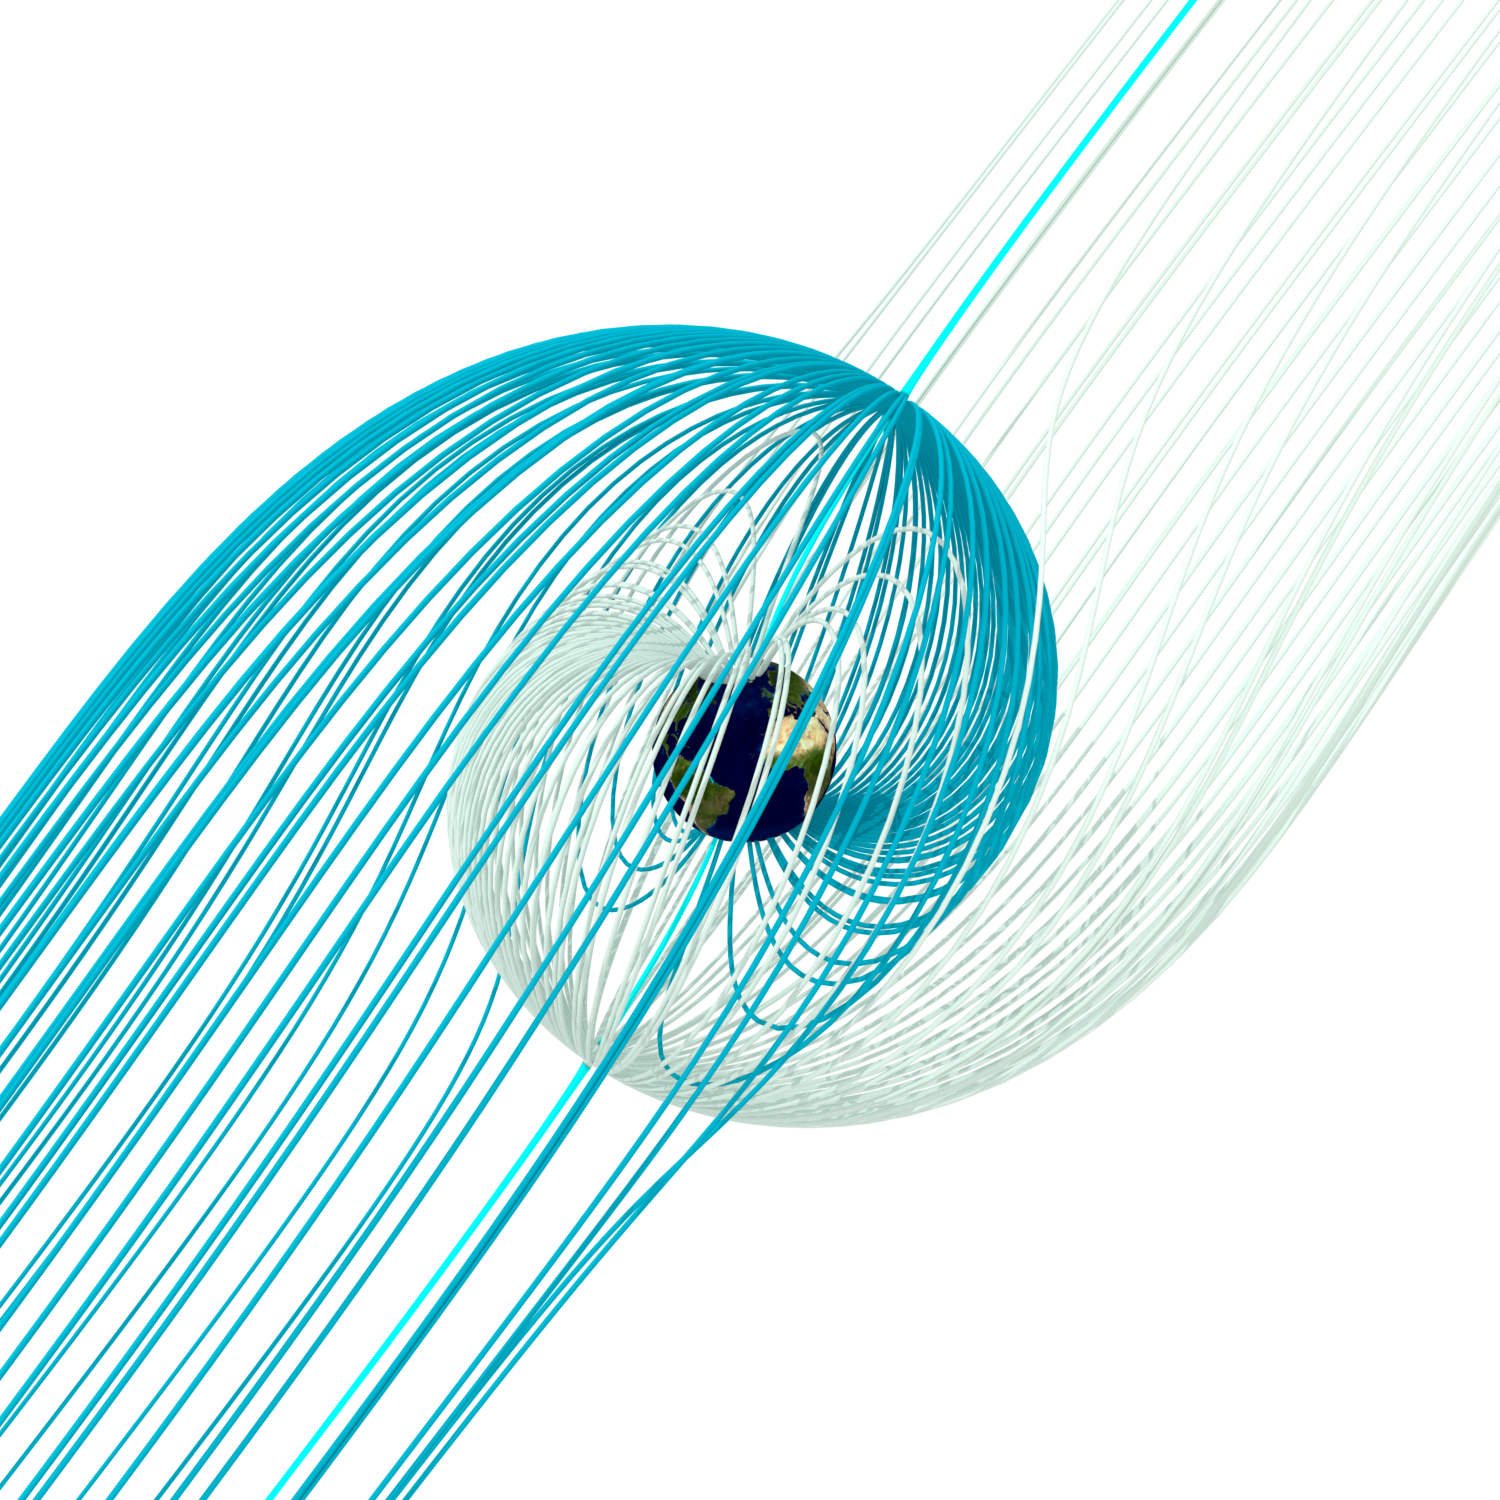
\includegraphics[width=\onecolwid]{fig/separatrix_dipole.png}
    \end{figure}

    The magnetic field of a dipole embedded in a guide field of direction $(-1,0,-1)$ is
    shown in the figure above. 
    The spines are colored cyan, whereas the spines are colored dark and light blue. 


\end{block}

%----------------------------------------------------------------------------------------

\end{column} % End of column 1.2

\end{columns} % End of the split of column 1
\end{column} % End of the first column

\begin{column}{\sepwid}\end{column} % Empty spacer column

\begin{column}{\onecolwid} % Begin the last column


%----------------------------------------------------------------------------------------
%
%----------------------------------------------------------------------------------------

\begin{block}{The Isotropic field}
    The function $g:\mathbb{R}^3\rightarrow S^2$ 
    is a mapping from a 3-dimensional space to a two-dimensional space.
    At any point in $\mathbb{R}^3$ (with exeption of null points and singularities), 
    there is a there is a direction in which the direction
    of the magnetic field remains constant. 
    We call these lines the isotropes of the magnetic field. 
    These lines cannot start or end, except at nulls. 

    Since the index of a null equals the degree of the mapping of $g|_\partial D^3_{x_0}$, 
    this means that at a null of index $\pm 1$, at least one isotrope corresponding to every
    direction is present on the surface of $D^3_{x_0}$. 
    Since this index theorem holds for any volume that encloses the null, these isotropes
    approach the null arbitrarily closely. 
    The isotropes  
    


\end{block}


\begin{block}{Calculating the Isotropic field}

The index of a null can be defined as the index of the map from a surface
enclosing the null to $S^2$ via $g$. This can be extended to a surface
enclosing several nulls. We would like to construct a vector field,
that when integrated over this surface, gives the sum of the indices of
the enclosed nulls. We define this by pulling back via $g$ the
integration over $S^2$ used to define the index to an integral over a
surface in $\mathbb{R}^3$.\\
	\begin{multline}
		4\pi\sum_{x_i\in U}\mathrm{Ind}(x_i)=\int_{g_*\partial U}\omega=\int_{g_*\partial U}d\alpha d\beta J(\alpha,\beta)\\
		=\int_{\partial U}dxdy
\begin{vmatrix}
  \partial_x\alpha & \partial_y \beta \\
  \partial_y\alpha & \partial_y \beta
\end{vmatrix}
	J(\alpha,\beta)\\
=\int_{\partial U}g^*\omega=\int_{\partial U}v\cdot da
	\end{multline}
Here we have taken some coordinates $(\alpha,\beta)$ on $S^2$, for which the
	area two-form on $S^2$ becomes $d\alpha\wedge d\beta J(\alpha,\beta)$.
	We find that the vector field, which we call the isotrope field, is the
	Hodge dual of the pullback over $f$ of the area two-form on $S^2$,
	\begin{equation}
		v=\star g^*\omega
	\end{equation}
for which we can find an expression in terms of our coordinates on $S^2$ as functions of
	$R^3$ defined by $g(x)=(\alpha(x),\beta(x))$. For any two vectors $a,b$:
	\begin{multline}
		v\cdot(a\times b)=g^*\omega(a,b)=
\begin{vmatrix}
  \partial_x\alpha & \partial_y \beta \\
  \partial_y\alpha & \partial_y \beta
\end{vmatrix}
J(\alpha,\beta)\\
		=(\nabla\alpha\times\nabla\beta)\cdot(a\times b)J(\alpha,\beta)
	\end{multline}
So $v$ can be written as:
	\begin{equation}
		v=(\nabla\alpha\times\nabla\beta)J(\alpha,\beta)
	\end{equation}
We can immediately see that $g$ is constant on streamlines of $v$, so the streamlines of $v$ are by definition the previously defined isotropes of $\mathbf{B}$.
	\begin{equation}
		v\perp\nabla\alpha,\nabla\beta\Rightarrow\partial_v\vec g=0
	\end{equation}
If we choose the usual angular coordinates on the sphere, $(\alpha,\beta)\Rightarrow(\theta,\phi)$, then
	\begin{equation}
		v=(\nabla\theta\times\nabla\phi)\sin\phi
	\end{equation}

    The Isotrope field is directed away from nulls of index $+1$ and towards nulls of
    index $-1$.
    In this sense the Isotrope field is analogous to the electric field of  point charges, and it's
    integral over a surface calculates the topological charge enclosed.



\end{block}

\begin{block}{Isotropes of a localized field embedded in a guide field}
    A localized magnetic field is a field generated by some local current distribution
    that goes to zero sufficiently rapidly at infinity. 
    Examples include the dipole field of a planet or star, or the currents carried by the
    plasma in an FRC. 
    Such local configurations are often embedded in a guide field, such as the
    interplanetary or galactic magnetic field, or the field produced by external coils in
    the case of the FRC. 

    The question then is, where and what types of nulls exist in this configuration of
    local field plus guide field. 
    At sufficient distance, the guide field is stronger than the local field, and the
    mapping of $g$ from the surface of a sufficiently large ball $D^3$ reduces to a null-homotopic
    function (degree 0).
    The indices of the nulls enclosed in this ball must therefore always sum to zero. 

    The isotropes of a local field
    constitute lines, which cannot end, and must therefore continue to infinity. 
    When the local field is placed in a guide field (direct sum of the two fields), the
    nulls appear on the isotrope corresponding with the direction opposite to the
    direction of the guide field. 
    The two fields sum to zero where the local field has equal magnitude to the guide
    field. 
    Surfaces of constant field strength are compact and closed, and the isotrope pierces
    them an even number of times, resulting in nulls of index +1 where the isotrope
    enters, and -1 where the isotrope leaves. 
    




\end{block}

%----------------------------------------------------------------------------------------

\begin{block}{References}

\nocite{*} % Insert publications even if they are not cited in the poster
\small{\bibliographystyle{unsrt}
\bibliography{refs}\vspace{0.75in}}

\end{block}

\begin{block}{Source}
This poster is available under the Apache licence 2.0 and all the source material is freely
available from the Github repository at \url{https://github.com/smiet/Topological_Nulls/}.

requirements:
\begin{itemize}
    \item Blender
    \item \LaTeX (beamer, qrcode)
    \item cmake
    \item Python: numpy, matplotlib
\end{itemize}

The entire poster including all rendered graphics are created by issuing the 'make' command.\\
\begin{centering}
    \qrcode[height=5cm]{https://github.com/smiet/Topological_Nulls}
\end{centering}

\end{block}

\end{column} % End of the second column

\begin{column}{\sepwid}\end{column} % Empty spacer column


\end{columns} % End of all the columns in the poster

\end{frame} % End of the enclosing frame

\end{document}
